\documentclass{assignment}
\ProjectInfos{高等量子力学}{PHYS5001P}{2022-2023 学年第一学期}{第四次作业}{截止时间: 2022 年  月  日 (周一)}{陈稼霖}[https://github.com/Chen-Jialin]{SA21038052}

\begin{document}
\begin{prob}[课本习题 2.24]
    考虑一维粒子被一个 $\delta$ 函数势
    \[
        V(x)=-\nu_0\delta(x),\quad(\nu_0\text{ 为正实数})
    \]
    束缚于一个固定的中心位置处, 求波函数和基态束缚能. 有激发的束缚态吗?
\end{prob}
\begin{prob}
    该粒子的哈密顿量为
    \begin{align}
        H=\frac{p^2}{2m}+V(x)=\left\{\begin{array}{ll}
            \frac{p^2}{2m},&x\neq 0,\\
            \frac{p^2}{2m}-\nu_0\delta(x),&x=0.
        \end{array}\right.
    \end{align}
    在 $x\neq 0$ 处的薛定谔方程为
    \begin{align}
        -\frac{\hbar^2}{2m}\frac{\partial^2\psi}{\partial x^2}=E\psi.
    \end{align}
    考虑到束缚态波函数在无穷远处的函数值为 $0$, $x<0$ 处和 $x>0$ 处波函数的通解分别为
    \begin{align}
        \psi(x<0)=Ae^{kx},\\
        \psi(x>0)=Be^{-kx},
    \end{align}
    其中 $k=\frac{\sqrt{2mE}}{\hbar}$.
    利用连续性条件
    \begin{gather}
        \psi(x=0^-)=A=\psi(x=0^+)=B,\\
        \psi'(x=0^+)-\psi'(x=0^-)=-Ak-Bk=\int_{0^-}^{0^+}\frac{\partial^2\psi}{\partial x'^2}\,\mathrm{d}x'=\frac{2m}{\hbar^2}\int_{0^-}^{0^+}[-\nu_0\delta(x)-E]\psi(0)\,\mathrm{d}x'=-\frac{2m\nu_0}{\hbar^2}A,
    \end{gather}
    解得
    \begin{align}
        A=B,\quad k=\frac{m\nu_0}{\hbar^2}.
    \end{align}
    考虑到波函数满足归一化条件, 得波函数
    \begin{align}
        \psi(x)=\frac{\sqrt{m\nu_0}}{\hbar}e^{-m\nu_0\abs{x}/\hbar^2},
    \end{align}
    基态束缚能为
    \begin{align}
        E=\frac{\hbar^2\Omega^2}{2m}.
    \end{align}

    该系统仅有一个束缚基态, 没有激发的束缚态
\end{prob}

\begin{prob}[课本习题 2.26]
    一个一维粒子 ($-\infty<x<\infty$) 受到一个可从
    \[
        V=\lambda x,\quad(\lambda>0)
    \]
    导出的恒力的作用.
    \begin{itemize}
        \item[(a)] 其能谱是连续的还是分立的? 写出由 $E$ 所确定的能量本征函数的近似表达式. 然后粗略地画出其示意图.
        \item[(b)] 简略地讨论, 如果用
        \[
            V=\lambda\abs{x}.
        \]
        代替 $V$, 什么地方需要改动?
    \end{itemize}
\end{prob}
\begin{sol}
    \begin{itemize}
        \item[(a)] 在 $x\rightarrow-\infty$ 处必有 $E>V$, 粒子非束缚, 故其能谱必为连续的.

        能量本征函数的近似表达式为
        \begin{align}
            \psi(x)\sim\left\{\begin{array}{ll}
                \frac{1}{[E-\lambda x]^{1/4}}e^{\pm\frac{i}{\hbar}\int_{-\infty}^x\sqrt{2m(E-\lambda x')}\,\mathrm{d}x'},&\text{for }x<\frac{E}{\lambda},\\
                \frac{1}{[\lambda x-E]^{1/4}}e^{-\frac{1}{\hbar}\int_{E/\lambda}^x\sqrt{2m(\lambda x'-E)}\,\mathrm{d}x'},&\text{for }x>\frac{E}{\lambda}.
            \end{array}\right.
        \end{align}
        如图 \ref{4-1} 所示.
        \begin{figure}[H]
            \centering
            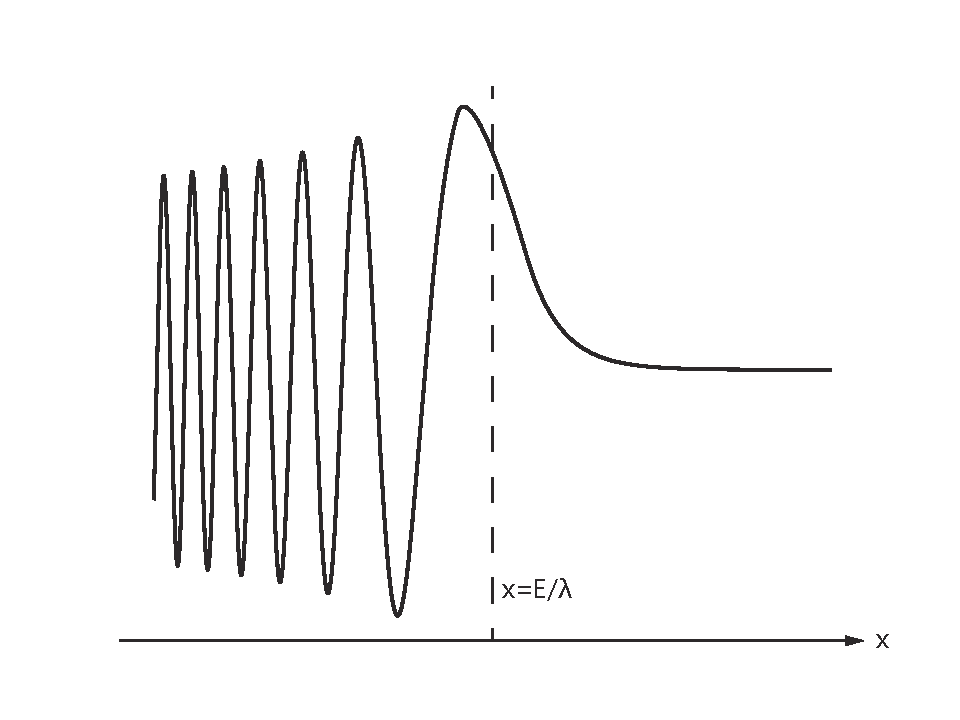
\includegraphics[width=.5\columnwidth]{4-1.pdf}
            \caption{能量本征函数的近似图像. 注意在 $x<E/\lambda$ 处波函数为波动形式, 且随着 $x\rightarrow-\infty$, 波动频率加快, 波动幅度变小; 在 $x>E/\lambda$ 处波函数为衰减形式.}
            \label{4-1}
        \end{figure}
        \item[(2)] 若 $V=\lambda\abs{x}$, 则粒子处于束缚态, 能谱为一系列分离的本征能量构成. 能量本征函数的近似表达式为
        \begin{align}
            \psi(x)\sim\left\{\begin{array}{ll}
                \frac{1}{[-\lambda x-E]^{1/4}}e^{\frac{1}{\hbar}\int_{-\infty}^x\sqrt{2m(-\lambda x'-E)}\,\mathrm{d}x'},&\text{for }x<-\frac{E}{\lambda},\\
                \frac{1}{[E-\lambda\abs{x}]^{1/4}}\cos\left[\frac{1}{\hbar}\int_{-E/\lambda}^x\sqrt{2m(E-\lambda\abs{x'})}\,\mathrm{d}x'\right],&\text{for }-\frac{E}{\lambda}<x<\frac{E}{\lambda},\\
                \frac{1}{[\lambda x-E]^{1/4}}e^{-\frac{1}{\hbar}\int_{E/\lambda}^x\sqrt{2m(\lambda x'-E)}\,\mathrm{d}x'},&\text{for }x>\frac{E}{\lambda},
            \end{array}\right.
        \end{align}
        或
        \begin{align}
            \psi(x)\sim\left\{\begin{array}{ll}
                \frac{1}{[-\lambda x-E]^{1/4}}e^{\frac{1}{\hbar}\int_{-\infty}^x\sqrt{2m(-\lambda x'-E)}\,\mathrm{d}x'},&\text{for }x<-\frac{E}{\lambda},\\
                \frac{1}{[E-\lambda\abs{x}]^{1/4}}\sin\left[\frac{1}{\hbar}\int_{-E/\lambda}^x\sqrt{2m(E-\lambda\abs{x'})}\,\mathrm{d}x'\right],&\text{for }-\frac{E}{\lambda}<x<\frac{E}{\lambda},\\
                \frac{1}{[\lambda x-E]^{1/4}}e^{-\frac{1}{\hbar}\int_{E/\lambda}^x\sqrt{2m(\lambda x'-E)}\,\mathrm{d}x'},&\text{for }x>\frac{E}{\lambda},
            \end{array}\right.
        \end{align}
        这些本征函数均为偶函数或奇函数.
        能量本征值满足
        \begin{align}
            \int_{-E/\lambda}^{E/\lambda}\sqrt{2m(E-\lambda\abs{x'})}\,\mathrm{d}x'=(n+\frac{1}{2})\pi\hbar,\quad n=0,1,2,3,\cdots
        \end{align}
        解得能量本征值为
        \begin{align}
            E_n=\frac{\left[3\left(n+\frac{1}{4}\right)\pi\hbar\lambda\right]^{2/3}}{2m^{1/3}},\quad n=0,1,2,3,\cdots
        \end{align}
    \end{itemize}
\end{sol}
\end{document}